\documentclass[10pt,a4paper]{book}
\usepackage{listings,graphicx,tikz,titlepic}

\title{Ardour Development Manual}
\titlepic{\includegraphics{graphics/ardour_bw.pdf}}
\author{}

\newcommand{\todo}[1]{\textbf{XXX --- #1}}
\newcommand{\code}[1]{\texttt{#1}}
\lstset{frame=single,language=c++,columns=fullflexible,basicstyle=\ttfamily,commentstyle=\footnotesize\textit,texcl=true,escapechar=\@,escapebegin=\footnotesize\itshape}
\begin{document}
\maketitle

\clearpage
\thispagestyle{empty}

\bigskip
\bigskip
\bigskip

\begin{quote}

\emph{``There is a theory which states that if ever anyone discovers
  exactly what the Universe is for, and why it is here, it will
  instantly disappear and be replaced by something even more bizarrely
  inexplicable.}

\smallskip

\emph{There is another theory which states that this has
  already happened.}

\smallskip

\emph{There is yet a third theory which suggests that
  both of the first two theories were concocted by a wily editor of
  `The Hitch-hikers' Guide to the Galaxy' in order to increase the
  level of universal uncertainty and paranoia, and so boost the sales
  of the guide.  This last theory is of course the most convincing,
  because `The Hitch-hikers' Guide to the Galaxy' is the only book in
  the whole of the known universe to have the words `don't panic'
  inscribed in large, friendly letters on the cover.''}

\smallskip

--- Douglas Adams, `The Hitch-hikers' Guide to the Galaxy'
\end{quote}

\chapter{Introduction}

Welcome to Ardour!  This manual is intended to give guidance in
Ardour's construction and how best to develop it.

\section{Contacting other developers}

By far the most useful means of communication with other Ardour users,
testers and developers is via IRC.  Connect to
\texttt{irc.freenode.org}, join the \texttt{\#ardour} channel and make
yourself acquainted!

\chapter{Code overview}

The vast majority of Ardour is written in C++.  

Ardour's code is split into several sections, which are summarised
below by their location in the source tree.

\begin{itemize}
\item \code{gtk2\_ardour} --- the GUI front-end, written using GTK2.
  GTK is accessed using gtkmm.
\item \code{libs/ardour} --- the back-end.  This is a the UI-agnostic
  `core' of Ardour, which can be used by different user interface
  front-ends.  Currently, only the GTK2 interface is supported, but
  once upon a time a keystroke-based interface to libardour also
  existed.
\item \code{libs/pbd} --- a library of useful miscellany.
\item \code{libs/evoral} --- a library for managing lists of events of
  various types, including automation and MIDI\@.
\item \code{libs/surfaces} --- code to support hardware control
  surfaces.
\end{itemize}

\chapter{The undo system}

Ardour allows unlimited undo / redo, and saves the undo stack with its
session.  This chapter describes how this is implemented.

\section{Overview}

The undo system employs similar principles to the way in which state
is saved in sessions.  C++ object state, and changes to that state, is
described with XML\@.  This has the advantage that it can easily be
serialized to and restored from disc.

There are two main approaches to saving undo state.  In some cases,
undo is performed by taking the full state of an object before some
operation, and then the full state afterwards, and storing both as
XML\@.  Undo and redo can then be achieved simply by setting state to
from the appropriate XML node.

In some cases, however, this approach can be inefficient.  Consider,
for example, a playlist with many thousands of regions.  If we want to
represent a region's addition to the playlist, the `full state'
approach means that we would take the state of all the regions both
before and after the region add.  This in turn means that a very large
`before' and `after' XML tree is required, which is inefficient both
in terms of storage space and also computation to save and restore
state.  For cases such as this, an alternative approach is taken: only
the \emph{differences} in the `before' and `after' state are stored.
In this way, rather than using a large state containing many regions,
we consider only a small state containing information about the single
added region.  This approach is much more efficient, and the cost of
some increased implementation complexity.

Classes that must be serialized to disc, and/or those that participate
in undo, inherit from \code{PBD::Stateful}.

\subsection{Commands}

However a change in state is described, it is represented by some
subclass of \code{PBD::Command}.  A change to some object represented
by `before' and `after' state is described by a
\code{PBD::MementoCommand}.  A change represented as a difference in
state is represented by a \code{PBD::StatefulDiffCommand}.  Since some
operation that is meaningful to the user may require changes to
several different Ardour objects, commands can be grouped into a
\code{PBD::UndoTransaction}.

Consider, as an example, the movement of two regions that are on
different tracks.  To the user, this is a single `move' operation.
Internally, however, there is a change to two different playlists.
Each playlist's change is described by a \code{StatefulDiffCommand},
and these commands are collected into a single \code{UndoTransaction}
which describes the operation that the user sees.

The \code{Session} assists somewhat in creation of
\code{UndoTransaction}s by keeping a `current' one
(\code{\_current\_trans}) and providing the
\code{begin\_reversible\_command} method to create a new
\code{UndoTransaction}, the \code{add\_command} method to add a
\code{Command} to the that \code{UndoTransaction}, and then the
\code{commit\_reversible\_command} method to add the finished
\code{UndoTransaction} to the history.


\section{Full state undo / redo}

In many cases, undo is achieved by keeping the entire state of an
object before some operation, then undoing it by setting that object
back to its pre-operation state.

The following is an example of how this is done:

\begin{lstlisting}
Object* foo;

// ...

// Tell the session that we are starting an undo-able operation
session->begin_reversible_command ("some operation");
// Obtain the state of the object foo now
XMLNode& before (foo->get_state ());
// Do some operation which changes the state of foo
foo->some_operation ();
// Obtain the new state of foo after the operation
XMLNode& after (foo->get_state ());
// Add a command to represent this change in state
session->add_command (
	new MementoCommand<Object> (*foo, &before, &after)
        );
// Commit any commands that have been added since
// begin\_reversible\_command as an undo transaction
session->commit_reversible_command ();
\end{lstlisting}

A single undo transaction is wrapped in calls to
\code{begin\_reversible\_command} and
\code{commit\_reversible\_command}.  Between these two calls, any
number of \code{Command} objects may be added to the undo transaction,
and they will all be undone as a single unit.

In this case, the \code{Command} is \code{MementoCommand}.  This is a
relatively simple class; it takes before and after XML state of an
object and keeps it with a pointer to the target object.  Undo is a
matter of calling \code{set\_state} on the object with the old state,
and redo calls \code{set\_state} with the new state.

\section{Diff-state (property-based) undo / redo}

This section describes undo / redo when it done using differences in
object state, rather than storing entire before and after states (much
of which may not have changed).  This can be more efficient in many
cases.


\subsection{Properties}

The most basic building block of the property-based undo system is the
\code{PBD::Property}.  This is a templated class which manages a
single piece of scalar state.  For example, \code{ARDOUR::Region}
contains the definition:

\begin{lstlisting}
PBD::Property<framepos_t> _position;
\end{lstlisting}

This declares a \code{Property} of type \code{framepos\_t}.  This
\code{\_position} can mostly be used as if it were a standard
variable, but the use of the \code{Property} class means that
\code{\_position} can also remember some history of previous values of
the position.  At the end of the following sequence of code:

\begin{lstlisting}
_position = 4;
_position->clear_changes ();
_position = 9;
\end{lstlisting}

the \code{\_position} property knows that its current value is 9, but
also that its previous value (before the last call to
\code{clear\_changes}) was 4.

\subsection{Stateful classes}

Classes such as \code{ARDOUR::Region} which have \code{PBD::Property}
members are derived from the class \code{PBD::Stateful}.  This helps
in managing the properties of its subclass.

\section{Example}

Consider a \code{Region} class which looks something like this:

\begin{lstlisting}
class Region : public Stateful {
    Property<framepos_t> _position;
    Property<framepos_t> _length;
};
\end{lstlisting}

and suppose we have an instance of this class called \code{region}
whose properties are set so that $\code{\_position} = 1$ and
$\code{\_length} = 2$.  We now want to change \code{\_position} and
\code{\_length} in an undo-able fashion.

\subsection{Making the changes}

Here's what happens when we do to make the changes:

\begin{lstlisting}
region->clear_changes ();
\end{lstlisting}

\code{Stateful::clear\_changes} calls \code{Property::clear\_changes}
on each of its properties (\code{\_position} and \code{\_length}).
This means that \code{\_position} and \code{\_length} clear their
\code{\_have\_old} flags.

\begin{lstlisting}
region->_position = 4;
region->_length = 6;
\end{lstlisting}

The properties update their current values and note their old values,
and the fact that they have been changed.

\begin{lstlisting}
session->add_command (new StatefulDiffCommand (region));
\end{lstlisting}

Finally we add a \code{StatefulDiffCommand} for the region that we
operated on.  This runs through the \code{Property} objects that the
region has, and asks each one if it has changed; if so the before- and
after- change values are noted in the \code{StatefulDiffCommand}.


\subsection{Sequence properties}

So far we have discussed diff-based undo / redo with simple scalar
properties.  Things get a little more complicated when we deal with
properties which themselves are lists of other \code{Stateful} items.

A typical example of this is Ardour's \emph{playlist}.  The playlist's
main piece of state is a list of regions, which themselves are
\emph{Stateful} objects.  We often want to be able to undo changes to
the contents of the list; ie things like addition or removal of
regions to or from the list.  Situations like this are particularly
well matched to the diff-based undo system; if there are 1000 regions
and we want to undo the addition of a single region, the diff-based
undo allows us to note details of just the one region, rather than the
1000 regions before and 1001 regions after.

A \code{SequenceProperty} is a subclass of \code{Property} which has a
container of objects.  It is templated on the container type, which
will typically be some STL class such as \code{vector} or \code{list}.
\code{SequenceProperty} can be used much like the container that it
wraps; it provides shim methods for things like addition, removal and
insertion of objects.  When these operations are performed,
\code{SequenceProperty} makes notes of the changes that have occurred,
much as \code{Property} does for its scalar state value.

Writing an undo record for a \code{SequenceProperty} is performed just
like that for any other \code{Property}.  Such undo records will
detail changes to the \emph{list} that the \code{SequenceProperty}
holds.  They will \emph{not}, by default, include details of any
changes to the items \emph{held} by the \code{SequenceProperty}.  Such
changes can, however, be included explicitly.  Consider some playlist,
whose constituent regions are to be changed by some operation.  We can
set up an undo record like this:

\begin{lstlisting}
playlist->clear_owned_changes ();
playlist->some_operation ();
vector<Command*> cmds;
playlist->rdiff (cmds);
session->add_commands (cmds);
\end{lstlisting}

Here we first see a call to \code{clear\_owned\_changes}, which is
similar to the usual call to \code{clear\_changes}, except that it
clears changes for the members of any \code{SequenceProperty} that
playlist contains.  In this case, \code{clear\_changes} will be called
for each region in the playlist.  \code{some\_operation} then
proceeds, perhaps making changes to the regions' state.  The call to
\code{rdiff} on the playlist collects \code{StatefulDiffCommand}s for
changes to any members of any of playlist's sequence properties (in
this case, changes to the regions).  These commands can then be added
to the session's undo stack in the usual way (there is a convenience
function \code{add\_commands} which adds multiple commands at the
same time.

Note that this code snippet does not consider any changes to the state
of playlist itself; if \code{some\_operation} may cause such changes,
the standard

\begin{lstlisting}
playlist->clear\_changes ();
playlist->some\_operation ();
session->add_command (new StatefulDiffCommand (playlist));
\end{lstlisting}

must \emph{also} be carried out to store this state.



\chapter{Threading}

Ardour runs multiple threads.  The main ones are as follows:

\begin{itemize}
\item \textit{GUI thread} --- where the GTK main loop runs.  All
  GUI-related code \textit{must} execute in this thread.
\item \textit{Process thread} --- code which that runs the JACK
  process callback.  This is where audio processing is done.
  Operations in this thread must not perform non-realtime operations
  such as allocating memory, as these could easily cause audio
  drop-outs.
\item \textit{Metering thread} --- a thread which computes peak values
  for meters based on the current fall-off settings.
\end{itemize}


\section{What the threads do}

\subsection{The GUI thread}

This runs the main GUI using GTK\@.  Any GUI-related or GTK call must
happen in this thread.  Long-running operations should not be carried
out in this thread, as blocking it will stop the GUI from responding.

\subsection{Process thread}

After some setup, the main body of the process thread is in
\code{AudioEngine::process\_callback}.  This method is called when
there audio / MIDI `work' to be done; typically it will be called when
there are $N$ frames of audio available from JACK (where $N$ is the
JACK block size).  This method takes the \textit{process lock},
\code{AudioEngine::\_process\_lock} which is held throughout the
callback.


\section{Cross-thread signalling}

Ardour makes much use of signal / slot messaging.  At its most basic
level, this system allows some class \code{Fred} to expose some
signal `Foo'.  Another class \code{Jim} can connect to
\code{Fred::Foo}, such that when \code{Fred} emits `Foo', a method
on \code{Jim} is called.  This is the system implemented by, for
example, \code{libsigc++} as used by \code{gtkmm}.  The main
conceptual advantage of this approach is that \code{Fred} need have
no dependency on \code{Jim} at all, and furthermore that another
class \code{Sheila} may also connect to the same signal, again
without \code{Fred} being any the wiser.

Using such a system across threads (so that, for example, the process
thread can signal the GUI thread) has some complications, chief
amongst which is that signal emissions from a given thread $A$ to $B$
must not block thread $A$ while they await processing.  In addition,
emission of signals from a process thread must be real-time safe.

Ardour's code to handle cross-thread signalling is based on (and
wraps) the \code{boost::signals2} library.

\subsection{The \code{Signal} class}

Ardour's basic `signal' class is \code{PBD::Signal}$N$, where $N$ is
the number of parameters that the signal has.  Consider, for example,
\code{PBD::Signal0}.  If a class \code{Fred} declares such a signal

\begin{lstlisting}
class Fred {
  PBD::Signal0<void> Foo;
};
\end{lstlisting}

then other classes can connect to the signal \code{Foo} using one of
the members of \code{Signal0}.

There are two main concerns with the connection of signals.  Consider
the case where \code{Fred} emits a signal that \code{Jim} connects to.
If \code{Jim} is destroyed, it is important that \code{Fred} stops
attempting to deliver signals to it.  Also, care is needed if the code
in \code{Jim} must be executed in a different thread to the one which
emitted the signal.

\subsubsection{Connection management}

Connecting to a signal results in the creation of a `connection'
object, represented in Ardour by \code{PBD::ScopedConnection}.  A
\code{ScopedConnection} is created during connection of a signal, and
its signal is disconnected when the \code{ScopedConnection} goes out
of scope.  Ardour also provides the \code{ScopedConnectionList}, which
a class can inherit from if it connects many signals.  The detailed
use of these classes is discussed in the following sections.

\subsubsection{Connecting to the same thread}

If the connected code is to be executed in the same thread as the
signal emission, connection is simple, so that:

\begin{lstlisting}
PBD::ScopedConnection c;
foo.connect_same_thread (c, boost::bind (&Jim::bar, this));
\end{lstlisting}

or

\begin{lstlisting}

class Fred : public PBD::ScopedConnectionList {
...
};

Fred cl;

foo.connect_same_thread (cl, boost::bind (&Jim::bar, this));
\end{lstlisting}

will result in \code{Jim::bar} being called when \code{foo} is
emitted.  The \code{connect\_same\_thread} method calls the boost
library directly.

The \code{c} and \code{cl} objects in the
examples above are a \code{ScopedConnection} and a
\code{ScopedConnectionList} respectively.  Details of the new
connection are filled into the \code{ScopedConnection} or added to the
\code{ScopedConnectionList}.

The interaction of the signal and the connection are perhaps best
illustrated with some code fragments:

\begin{lstlisting}
class Foo {
public:
  void fred () {
    A ();
  }

  PBD::Signal0<void> A;
};

class Bar {
public:
  void Bar (Foo* f) {
    f->A.connect_same_thread (
        _connection, boost::bind (&Bar::sheila, this)
      );
  }

  void sheila () {
    ...
  }
};

private:
  PBD::ScopedConnection _connection;
};

Foo* f = new Foo;

// Make a new Bar and its constructor will connect to Foo
Bar* b = new Bar (f);

// Foo::fred emits A, which results in Bar::sheila being called
f->fred ();

// Deleting b means that Bar::\_connection is also deleted, which
// disconnects the connection made to Foo::A in Bar's constructor.
delete b;

// Foo::fred emits A as before, but no-one is listening!
f->fred ();
\end{lstlisting}

If \code{Bar} is larger, and connects to more signals, it may be more
convenient to modify the code above to:

\begin{lstlisting}
class Foo {
public:
  void fred () {
    A ();
  }

  PBD::Signal0<void> A;
};

class Bar : public PBD::ScopedConnectionList {
public:
  void Bar (Foo* f) {
    f->A.connect_same_thread (
        *this, boost::bind (&Bar::sheila, this)
      );
  }

  void sheila () {
    ...
  }
};
\end{lstlisting}

In this case, the connection is stored in the parent
\code{ScopedConnectionList} class, and disconnected when it is
destroyed.  This approach requires less code in many cases.

\subsubsection{Connecting to a different thread}

In one case, the emission of signals from the back-end to a user
interface (UI), it is necessary to have the signal handler running in
a different thread to the emission.  Connecting signals in this way is
quite similar to connecting same-thread signals, although the
implementation is more complicated.

Ardour has several components which it considers UI\@.  The most
obvious, perhaps, is the graphical UI; other components are the Open
Sound Control (OSC) interface, and also those provided by hardware
control surfaces.

In the Ardour code, each of these UIs inherits from \code{AbstractUI},
which in turn is-a \code{BaseUI} which is-a \code{EventLoop}, as shown
in Figure~\ref{fig:ui-class-hierarchy}.

\begin{figure}[ht]
\begin{center}
\include{graphs/ui-class-hierarchy}
\end{center}
\caption{The class hierarchy for UI classes}
\label{fig:ui-class-hierarchy}
\end{figure}

Consider first how the Ardour code sets up a connection to a signal
which is emitted in one thread and responded to in another.  In the previous
listing from the single-threaded case, the code to make the connection is

\begin{lstlisting}
    f->A.connect_same_thread (
        _connection, boost::bind (&Bar::sheila, this)
      );
\end{lstlisting}

This connects \code{Bar::sheila} to a signal \code{A} on the object
\code{f}.  When \code{A} is emitted, \code{Bar::sheila} will be run in the
thread from which \code{A} was emitted.

In the case where \code{A} is emitted in a non-UI thread, and must be
handled by code in a UI thread, the connection code must be modified as
follows:

\begin{lstlisting}
    f->A.connect (
        _connection, invalidator (), boost::bind (&Bar::sheila, this), gui_thread ()
      );
\end{lstlisting}

As before, we have a \code{\_connection} object to hold details of the connection, and
a \code{boost::bind} to the function that must be called on signal emission.  There
are two additions; an `invalidator', and an indication of the thread that \code{Bar::sheila}
must be called in.  These extra parts will be discussed shortly.

\subsubsection{The mechanics of cross-thread signalling}

In the single-threaded case, Ardour simply connects the signal to the slot using the Boost
library's mechanisms.  On emission of the signal, the slots are called directly.

In the multi-threaded case, consider the case where some back-end
thread $A$ raises a signal that some UI thread $B$ needs to respond to.

\begin{enumerate}
\item Ardour connects the signal to \code{EventLoop::call\_slot} on
  the receiving \code{EventLoop}.  This is a pure virtual method
  implemented by \code{AbstractUI}.  Hence when the signal is emitted
  in thread $A$, \code{AbstractUI::call\_slot} is called in $A$.
\item \code{AbstractUI::call\_slot} obtains a \code{RequestObject} by
  calling \code{AbstractUI::get\_request}.
\begin{enumerate}
\item \code{AbstractUI::get\_request} checks to see if thread $A$ has
  a per-thread request buffer (a ring-buffer set up by
  \code{AbstractUI::register\_thread}).
\item If so, \code{get\_request} returns the next available write
  space in the per-thread buffer; otherwise it returns a
  \code{RequestObject} allocated by \code{new}.
\end{enumerate}
\item \code{AbstractUI::call\_slot} sets up the \code{RequestObject}
  with details of the slot that is to be called, and passes it to
  \code{AbstractUI::send\_request}.
\item If thread $A$ has a per-thread request buffer, the write pointer
  on the ringbuffer is incremented to `commit' the
  \code{RequestObject} to the buffer; otherwise the
  \code{RequestObject} is written to \code{AbstractUI::request\_list}.
\item \code{BaseUI::request\_channel} is signalled to indicate that a
  request is waiting.
\end{enumerate}

Now, in thread $B$:

\begin{enumerate}
\item \code{BaseUI::request\_channel} calls \code{BaseUI::request\_handler}.
\item This calls \code{AbstractUI::handle\_ui\_requests}.
\item This looks in each of its request buffers (there will be one for
  each thread which called \code{AbstractUI::register\_thread}) and calls the requested slots.
\item It then looks in the \code{AbstractUI::request\_list} and calls those slots.
\end{enumerate}


\subsubsection{Invalidation}

Consider the case where an object \code{f} of class \code{Fred} has a
cross-thread connection to a signal on some object \code{j}.  Should
\code{f} connect to \code{j} and subsequently be destroyed, the
aforementioned \code{ScopedConnection} or \code{ScopedConnectionList}
would typically also be destroyed, removing the connection.  There is
a complication, however, in the cross-thread case due to the
disconnect between the signal being emitted and handled.  Consider the
following pathological case:

\begin{enumerate}
\item Object \code{f} of class \code{Fred} connects to some signal on some object \code{j}.
\item \code{j} emits the signal; a \code{RequestObject} gets queued up.
\item \code{f} is destroyed; the connection between \code{f} and
  \code{j} is removed, but alas too late.
\item The \code{RequestObject} gets processed by the event loop of the
  UI that \code{f}'s signal handler runs in; this results in some
  method being called on \code{f}.
\item \code{f} has been destroyed, so bad things happen.
\end{enumerate}

To deal with this problem, a cross-thread connection is supplied with
an \emph{invalidation record}.  This is an object of type
\code{PBD::InvalidationRecord} which is usually created by a helper
function such as \code{Gtkmm2ext::\_\_invalidator} (wrapped in the macro
\code{invalidator()}).

The \code{InvalidationRecord} is kept in the \code{RequestObject}.
The \code{Gtkmm2ext::\_\_invalidator} connects to a given
\code{sigc::trackable}'s \code{add\_destroy\_notify\_callback} and
calls \code{EventLoop::invalidate\_request} on receipt.  For our
example, this means that when \code{f} is destroyed the UI's
\code{EventLoop::invalidate\_request} is called.  This in turn sets
all \code{RequestObject}s for this \code{InvalidationRecord} to be
invalid, so that they are not called.

In other words, the following sequence occurs:
\begin{enumerate}

\item We make a connection using something like
\begin{lstlisting}
void Fred::frobozz () {
  j.foo.connect (
    _c, invalidator (*this),
    bind (&Fred::bar, this), gui_thread ());
}
\end{lstlisting}
\begin{enumerate}
\item \code{invalidator()} (ie \code{Gtkmm2ext::\_\_invalidator}) creates an \code{InvalidationRecord}.
\item \code{j.foo} is attached to \code{EventLoop::call\_slot}
\end{enumerate}

\item \code{j.foo} is emitted.
\begin{enumerate}
\item \code{EventLoop::call\_slot} is called.
\item A \code{RequestObject} is made, and the \code{InvaldationRecord} is made to point to it.
\item The \code{RequestObject} is put into the request buffer.
\end{enumerate}

\item The object of type \code{Fred} is deleted.
\begin{enumerate}
\item \code{EventLoop::invalidate\_request} is called via \code{Fred}'s \code{sigc::trackable} base's \code{destroy\_notify\_callback}.
\item This marks the \code{RequestObject} as invalid.
\end{enumerate}

\item When \code{j}'s event loop runs, the \code{RequestObject} is
  ignored as it has been marked invalid; the destroyed \code{Fred}
  object is not called, and all is well.

\end{enumerate}

\section{How signals get from disk to JACK outputs}

[midi]

Process thread: route / track calls diskstream::get\_playback, and then process\_output\_buffers on that.

Diskstream::get\_playback reads from its ringbuffer.


Butler thread: calls Track::do\_refill which in turn calls Diskstream::do\_refill

MidiDiskstream::do\_refill calls MidiDiskstream::read which calls MidiPlaylist::read

Assuming there's only 1 region, this calls Region::read\_at

Which reads from its source, which gets from the model, if there is one, or gets direct from the SMF.



%%%

CrossThreadPool: is-a Pool.

PerThreadPool: manages a CrossThreadPool per thread.  create\_per\_thread\_pool
called by SessionEvent::create\_per\_thread\-pool

---

%%%


\chapter{The process thread}

When JACK asks us to do stuff, we run the process thread.  The
singular `thread' in its name is somewhat historic, as newer version
of Ardour (3 and beyond) support multi-threaded processing.  This
allows Ardour to take advantage of multi-core CPUs.

\section{Example session}

We have tracks $T_1$ and $T_2$ and busses $B_1$, $B_2$ and $B_3$.  All
busses feed $M$.  $T_1$ feeds $B_1$, $T_2$ feeds $B_2$, $B_2$ feeds
$B_3$.

% drawing!

\section{The route graph}

\subsection{Route fed-by sort}

Setup done by \code{Graph::rechain}.  This is passed a list of routes
in order from beginning to end of the chain, so for our example it is:

\begin{itemize}
\item $A_1$
\item $A_2$
\item $B_1$
\item $B_2$
\item $B_3$
\item $M$
\end{itemize}

ie anything that feeds something else is before it in the list.

\subsection{Graph setup}

We make a list \code{\_nodes\_rt} that is a list of routes.

Then for each node (ie route):

\begin{itemize}
\item Set \code{has\_output} to true if it feeds anything.
\item Set \code{has\_input} to true if it is fed by anything.
\item Add any route that we directly feed to \code{\_activation\_chain}.
\end{itemize}

\chapter{Export}

Ardour's export facilities are comprehensive, and the code that
implements them is rather complex.  This chapter describes that export code.

\section{Capabilities}

Export has a number of parameters.  To summarise, these are:

\begin{itemize}
\item \textbf{Format}
  \begin{itemize}
  \item File format (AIFF, WAV, Ogg Vorbis etc.)
  \item Sample rate.
  \item Type of sample rate conversion, if required.
  \item Normalization
  \item Trimming of silence.
  \item Bit depth.
  \item Type of dithering, if required.
  \end{itemize}
\item \textbf{Exported file locations and names}; where to put the exported files and what to call them.
\item \textbf{Time ranges} to export.
\item \textbf{Tracks and/or busses} to export.
\end{itemize}



Export Formats

Described by subclass of ExportFormat.  Subclasses are:

ExportFormatLinear : AIFF, AU, IRCAM, WAV, W64, RAW.
ExportFormatOggVorbis
ExportFormatFLAC
ExportFormatBWF

ExportFormatBase 

This is:
 format id (F\_WAV, F\_W64, F\_AIFF, F\_AU, F\_IRCAM, F\_RAW, F\_FLAC, F\_Ogg)
 quality (LosslessLinear, LosslessCompression, LossyCompression)
 sample format (8-bit, 16-bit, 24-bit, 32-bit, U8, float, double, Vorbis)


\chapter{Miscellany}

\section{Time}

\begin{quote}
\emph{``Time is an illusion caused by the passage of history; history is an illusion caused by the passage of time.'', Douglas Adams}

\medskip

\emph{``Tempora mutantur et nos mutamur in illis'', Lothair I (attr.)}
\end{quote}

\subsection{Expressions of time intervals}

Ardour has a couple of ways of representing an interval of time, and
some mechanisms to convert between the two representations.

The first is the \emph{frame}.  This is a period of time equal to
$1/F_S$, where $F_S$ is the sampling rate of the session.  Life is
simple with the frame, as its duration is constant throughout the
timeline. 

There is also the more complicated \emph{beat}.  This is defined
within Ardour as a unit of time that is related to tempo, such that a
beat length $b$ in seconds is given by

\begin{equation}
b = \frac{60}{T}
\end{equation}

where $T$ is the tempo in beats per minute.  The tempo of a session
can change multiple times within a session.  This means that, for
example, a period of $B$ beats in one part of the session may
correspond to a different number of seconds depending on whereabouts
the period is within the session.


\subsection{Durations, offsets and session positions}

Many confusions and bugs arise from misunderstandings of times
represented as intervals from some reference point.  There are a few common situations within Ardour:

\begin{itemize}
\item \emph{Session frames} --- it is common to express some time as
  an interval in frames from the start of the session (i.e.\ $0$ on
  the timeline, the leftmost point in the editor, not the session
  `start' location marker).  The intention is to use the type
  \code{framepos\_t} for such times.  Comments often refer to times
  like this as being in `session frames'.
\item \emph{Region-offset positions} --- it is also common to express
  things as being at some time within a region.  This usually means
  that the `position' is an interval from the \emph{position} property
  of the region, which in itself is stored in session frames.
\item \emph{Source-offset positions} --- since a region can start at
  any point within its source, it is also fairly common to express
  times as being offset from the start of a region's source.
\end{itemize}

Figure~\ref{fig:times-with-regions} is an attempt to clarify some of
these ideas.  Consider this region, thinking of all time intervals as
being in frames.

\begin{figure}[ht]
\begin{center}
%\includegraphics{diagrams/times_with_regions.pdf}
\end{center}
\caption{Some expressions of times within Ardour}
\label{fig:times-with-regions}
\end{figure}

The figure shows a thick black line to represent session $0$.  We then
have some event `Fred', whose time can be expressed most simply in
\emph{session frames} as $f$.  We then have a region, coloured in
blue.  This has a \emph{position} property, expressed in session
frames as $p$.  Its source is coloured grey, and we can see that this
region starts at an interval $s$ into its source (so that the region's
\emph{start} property is $s$).  If `Fred' is in some way related to
  this region, we can express its time in new ways: as an offset from
  the region position, $g$, or as an offset from the source start,
  $h$.

It goes without saying that confusing any of these representations of
where `Fred' is will cause problems.



\end{document}

